\chapterimage{chapter_head_2.pdf} % Chapter heading image

\chapter{\textcolor{blue}{Tecnicas para a musicalidade}}




%%%%%%%%%%%%%%%%%%%%%%%%%%%%%%%%%%%%%%%%%%%%%%%%%%%%%%%%%%%%%%%%%%%%%%%%%%%%%%%%
%%%%%%%%%%%%%%%%%%%%%%%%%%%%%%%%%%%%%%%%%%%%%%%%%%%%%%%%%%%%%%%%%%%%%%%%%%%%%%%%
\section{\textcolor{red}{Mickey mousing}}
\index{Musicalidade!Mickey mousing}
onomatopeia andante


%%%%%%%%%%%%%%%%%%%%%%%%%%%%%%%%%%%%%%%%%%%%%%%%%%%%%%%%%%%%%%%%%%%%%%%%%%%%%%%%
%%%%%%%%%%%%%%%%%%%%%%%%%%%%%%%%%%%%%%%%%%%%%%%%%%%%%%%%%%%%%%%%%%%%%%%%%%%%%%%%
\section{\textcolor{red}{Leitmotif}}
\index{Musicalidade!Leitmotif}
motivo principal \cite[pp. 7]{bribitzer2015understanding} \cite[pp. 465]{apel1969harvard}


%%%%%%%%%%%%%%%%%%%%%%%%%%%%%%%%%%%%%%%%%%%%%%%%%%%%%%%%%%%%%%%%%%%%%%%%%%%%%%%%
%%%%%%%%%%%%%%%%%%%%%%%%%%%%%%%%%%%%%%%%%%%%%%%%%%%%%%%%%%%%%%%%%%%%%%%%%%%%%%%%
\section{\textcolor{red}{Aspectos da musicalidade na dança}}
\subsection{\textcolor{red}{Dançar no pulso}}
Ver Figura \ref{fig:lamentoconsolopulso1}.
\begin{sidewaysfigure}
    \centering
    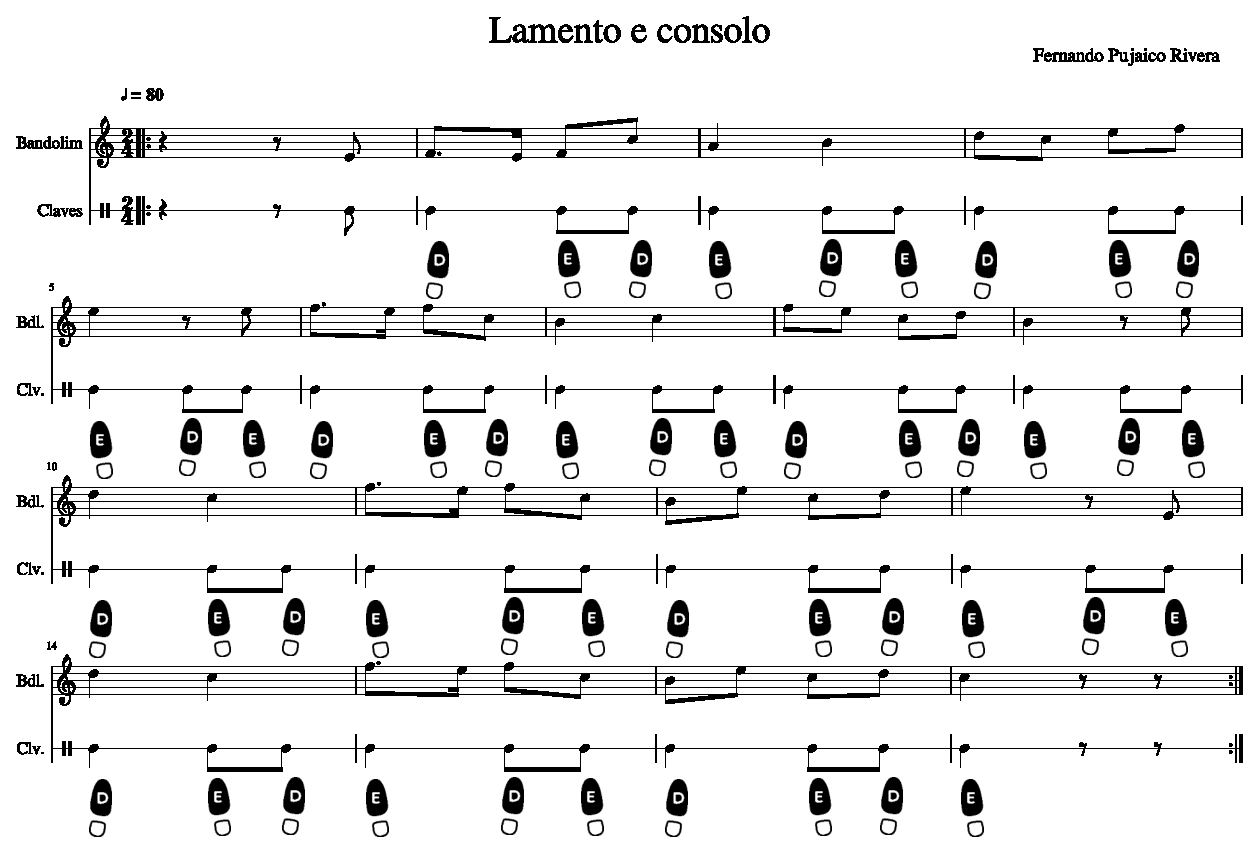
\includegraphics[width=\textwidth]{chapters/cap-musicalidade-tecnica/lamento-e-consolo-clave-pulso-1.eps}
    \caption{Música dançada no pulso.}
    \label{fig:lamentoconsolopulso1}
\end{sidewaysfigure}

Ver Figura \ref{fig:lamentoconsolopulsobreak1}.
\begin{sidewaysfigure}
    \centering
    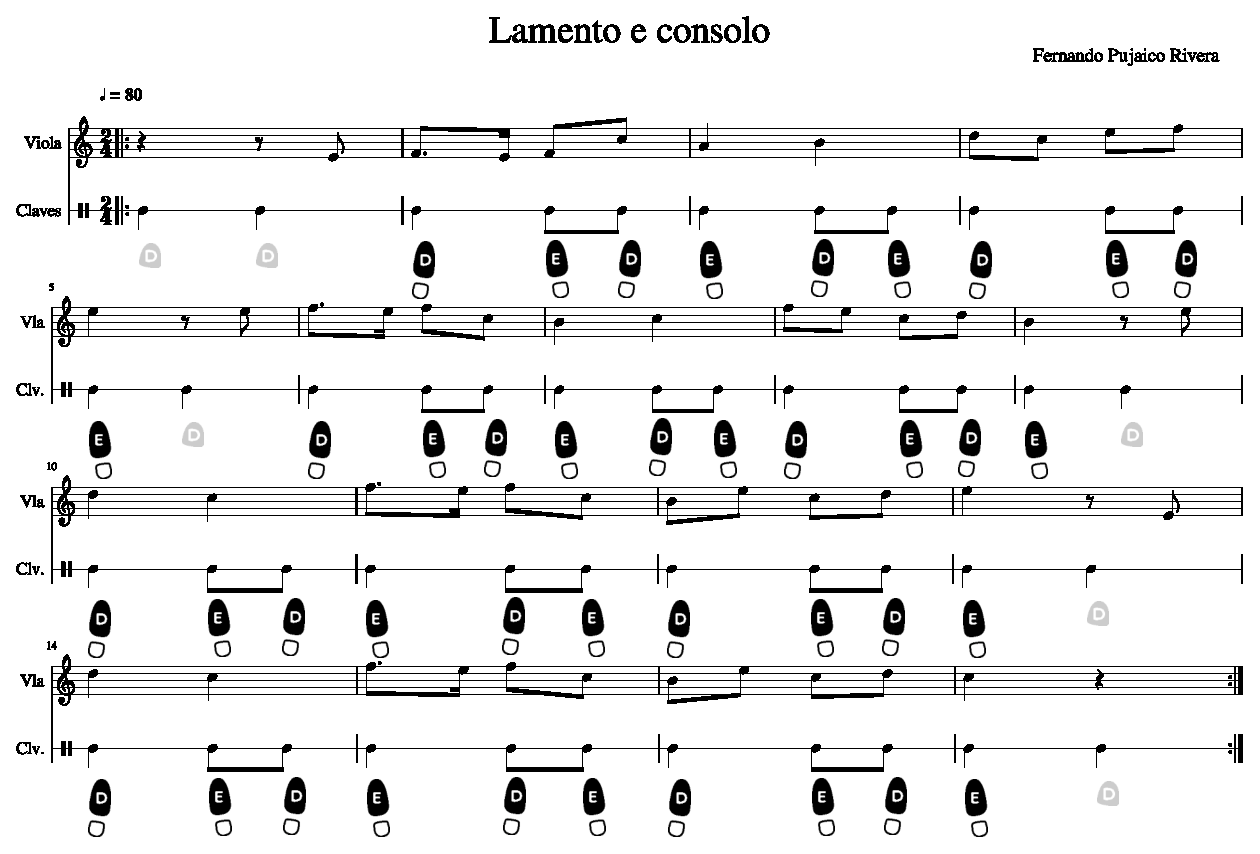
\includegraphics[width=\textwidth]{chapters/cap-musicalidade-tecnica/lamento-e-consolo-clave-pulso+break-1.eps}
    \caption{Música dançada no pulso e usando breaks.}
    \label{fig:lamentoconsolopulsobreak1}
\end{sidewaysfigure}


\subsection{\textcolor{red}{Dançar no ritmo}}
Una buena regla general, especialmente si es nuevo en el baile, es mantener el pulso o el ritmo en su cuerpo.

Mantener el pulso o el ritmo en la cabeza o en el pecho es una de las cosas más fáciles para cualquier persona.

%https://tangowords.wordpress.com/2017/01/10/elements-of-musicality-beat-and-rhythm/
\begin{comment}
quando começamos a dançar, aprendemos a dançar com o batida, 
depois de um tempo começamos a dançar com o ritmo, eventualmente descobrimos como dançar com a música. 
Claro, estes não são separados; Quando dançamos ao ritmo, 
também dançamos ao  batida. 
E quando dançamos a música, os elementos de batida e ritmo também estão lá.

Ao falar com os dançarinos, acho que às vezes há confusão entre batida e ritmo. 
Simplificando, a batida é o pulso constante que você sente na melodia, 
como um tique-taque do relógio. É com o que você pode bater palmas ou bater o pé em. 
O ritmo é o padrão real que as notas de comprimentos diferentes fazem, 
que em uma música podem ser as mesmas que os padrões de palavras. 
Além do tamanho das notas, o ritmo também é criado quando algumas notas são enfatizadas sobre outras.

Geralmente, a dance music (exceto valsa / vals, claro) tem quatro batidas no bar. 
As batidas 1 e 3 são as batidas fortes (o compás no tango) as batidas 2 e 4 
são as batidas fracas (às vezes chamadas de batidas de costas ou de batidas). 
Em seu nível mais simples, quando dançamos, tendemos a pisar nas batidas 1 e 3. 
(Embora, ao bater palmas, a preferência seja aplaudir a batida de trás).

Claro, tudo isso se aplica a qualquer dança criativa de parceiros, 
não apenas ao tango. Em algumas aulas, às vezes você ouve: 
"Este é um movimento de seis batidas" ou "Este é um movimento de doze batidas". 
Isso só é verdade se você estiver se limitando a dançar mecanicamente e unicamente 
ao batida da música. Se você está dançando ao ritmo, 
quantas batidas levará dependendo de como você trabalha com a música.

É muito fácil cair na armadilha de pensar em padrões de passos e se tornar um 
"dançarino de um e três". (E, infelizmente, a batida fortemente acentuada de boa 
parte do que se passa por dance music tende a encorajar isso ... mas isso é outra 
história para outro post no blog!) Somos dançarinos, não metrônomos.
\end{comment}

Ver Figura \ref{fig:lamentoconsoloritmo1}.
\begin{sidewaysfigure}
    \centering
    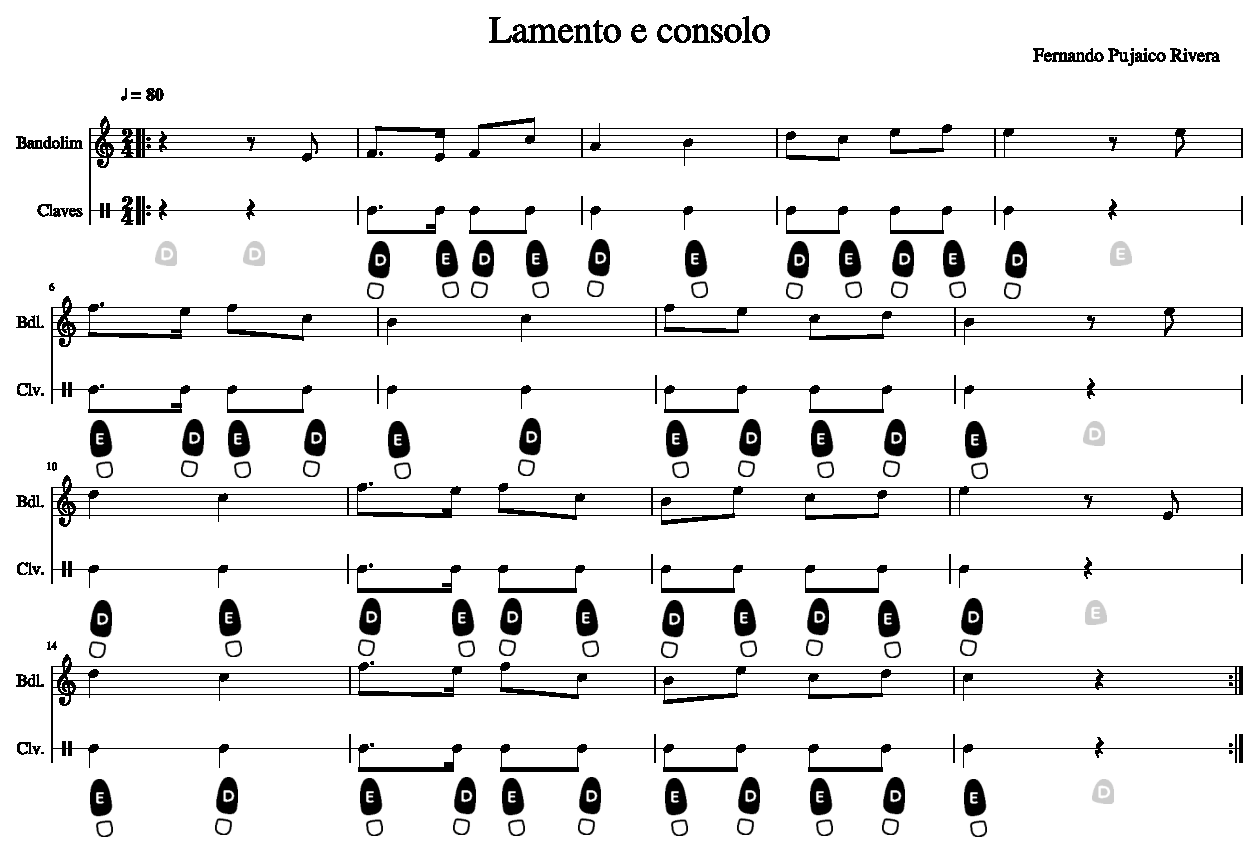
\includegraphics[width=\textwidth]{chapters/cap-musicalidade-tecnica/lamento-e-consolo-clave-ritmo-1.eps}
    \caption{Música dançada no ritmo.}
    \label{fig:lamentoconsoloritmo1}
\end{sidewaysfigure}

\subsection{\textcolor{red}{Dançar na melodia}}
Para darle un poco más de libertad y creatividad, 
mantener el pulso o el ritmo en sus pies le brinda la capacidad de interpretar 
la melodía con el resto de su cuerpo, si así lo desea.

\subsection{\textcolor{red}{Dançar na música}}

%%%%%%%%%%%%%%%%%%%%%%%%%%%%%%%%%%%%%%%%%%%%%%%%%%%%%%%%%%%%%%%%%%%%%%%%%%%%%%%%
%%%%%%%%%%%%%%%%%%%%%%%%%%%%%%%%%%%%%%%%%%%%%%%%%%%%%%%%%%%%%%%%%%%%%%%%%%%%%%%%
\section{\textcolor{red}{Seguindo isoladamente os instrumentos}}
Seria uma forma de mickey mousing
\begin{itemize}
\item Dançando choro-chorinho no ritmo esquecendo o ``Tchic-Tchic Tum''.
\item Trabalhando com marionetas um em cada mão, ou dedo.
\item Cada aluno simula que tem um instrumento virtual e toca ele.
\end{itemize}

%%%%%%%%%%%%%%%%%%%%%%%%%%%%%%%%%%%%%%%%%%%%%%%%%%%%%%%%%%%%%%%%%%%%%%%%%%%%%%%%
%%%%%%%%%%%%%%%%%%%%%%%%%%%%%%%%%%%%%%%%%%%%%%%%%%%%%%%%%%%%%%%%%%%%%%%%%%%%%%%%
\section{\textcolor{red}{Embolada, Rap e musicalizar poesias}}
\index{Musicalidade!Frase musical}
% https://scielo.conicyt.cl/scielo.php?script=sci_arttext&pid=S0719-32622018000100030
Figura \ref{rap:emocional-protesto1}

\begin{figure}[H]
\centering
\begin{abc}[name=abc-emocional-protesto1]
X: 1 % start of header
K: C stafflines=1 % scale: C major
M: 2/4 %meter - compasso
Q:1/4=100
V:1 clef=perc stem=up %name="Pauta com clave de fá"   sname="Pauta com clave de fá"
[V:1] |:!>!B3/2 B/2 B1 B1| B3/2 B/2 B1 B1 | B2 B2| B2 B1 B1:|
\end{abc}
\caption{Frase de 8 tempos, com palavra final grave.}
\label{rap:emocional-protesto1}
\end{figure}


\begin{citando}
Vida simples, metáfora de um corpo;\\
luzes cobertas, as lágrimas expostas.\\
Vida simples, luta contra o tempo;\\
brilha, existe, e terás respostas.\\
\end{citando}


Tabela \ref{tab:verso1}

\begin{table}[h!]
\begin{center}
\begin{tabular}{|l||l||l||l|} % 
\hline
compasso 1 & compasso 2   & compasso 3   & compasso 4 \\ \hline \hline
\textbf{Vi}da       & \textbf{sim}ples, me- & \textbf{tá}fora de um  & \textbf{cor}po;  \\ \hline
\textbf{lu}zes  co- & \textbf{ber}tas, as   & \textbf{lá}grimas ex-  & \textbf{pos}tas. \\ \hline
\textbf{Vi}da       & \textbf{sim}ples,     & \textbf{lu}ta contra o & \textbf{tem}po;  \\ \hline
\textbf{bri}lha, e- & \textbf{xis}te,       & \textbf{e} terás res-  & \textbf{pos}tas. \\ \hline
\end{tabular}
\caption{Verso 1.}
\label{tab:verso1}
\end{center}
\end{table}


Figura \ref{rap:emocional-protesto2}

\begin{figure}[H]
\centering
\begin{abc}[name=abc-emocional-protesto2]
X: 1 % start of header
K: C stafflines=1 % scale: C major
M: 2/4 %meter - compasso
Q:1/4=100
V:1 clef=perc stem=up %name="Pauta com clave de fá"   sname="Pauta com clave de fá"
[V:1] |:!>!B3/2 B/2 B1 B1| B3/2 B/2 B1 B1 | B2 B2| B2 z2:|
\end{abc}
\caption{Frase de 8 tempos, com palavra final aguda.}
\label{rap:emocional-protesto2}
\end{figure}

